\documentclass{article}
\usepackage{float}
\usepackage{textcomp}
\usepackage{graphicx}
\usepackage{booktabs}
\usepackage{color}
\usepackage{verbatim}
\usepackage{listings}
\usepackage{underscore}
\usepackage{amsmath}
\usepackage{amssymb}
\usepackage{listings}
% Define Language
\lstdefinelanguage{pseudocode}
{
  % list of keywords
  morekeywords={
	end, begin, for, end-for, if, end-if, do, then, else, return, read, to
  },
%  literate=%
%    {:}{$\colon$}1
%    {|}{$\bullet$}1
%    {==}{$=$}1
%    {=}{$=$}1
%    {!=}{$\neq$}1
%    {&&}{$\land$}1
%    {||}{$\lor$}1
%    {<=}{$\le$}1
%    {>=}{$\ge$}1
%    {all}{$\forall$}1
%    {exists}{$\exists$}1
%    {!in}{$\not\in$}1
%    {\\in}{$\in$}1
%    {=>}{$\implies$}2
%    ,
  sensitive=false, % keywords are not case-sensitive
  morecomment=[l]{//}, % l is for line comment
  morecomment=[s]{/*}{*/}, % s is for start and end delimiter
  morestring=[b]" % defines that strings are enclosed in double quotes
}

% Define Colors
\usepackage{color}
\definecolor{eclipseBlue}{RGB}{42,0.0,255}
\definecolor{eclipseGreen}{RGB}{63,127,95}
\definecolor{eclipsePurple}{RGB}{127,0,85}
 
% Set Language
\lstset{
  language={pseudocode},
  basicstyle=\small\ttfamily, % Global Code Style
  captionpos=b, % Position of the Caption (t for top, b for bottom)
  extendedchars=true, % Allows 256 instead of 128 ASCII characters
  tabsize=2, % number of spaces indented when discovering a tab 
  columns=fixed, % make all characters equal width
  keepspaces=true, % does not ignore spaces to fit width, convert tabs to spaces
  showstringspaces=false, % lets spaces in strings appear as real spaces
  breaklines=true, % wrap lines if they don't fit
  frame=trbl, % draw a frame at the top, right, left and bottom of the listing
  frameround=false, % make the frame round at all four corners
  framesep=4pt, % quarter circle size of the round corners
  numbers=left, % show line numbers at the left
  numberstyle=\tiny\ttfamily, % style of the line numbers
  commentstyle=\color{eclipseGreen}, % style of comments
  keywordstyle=\color{eclipsePurple}, % style of keywords
  stringstyle=\color{eclipseBlue}, % style of strings
}
%\usepackage{showkeys}
%\usepackage{float} % here for H placement parameter
\usepackage{flafter} 
\setcounter{secnumdepth}{5}
\usepackage[bookmarks=true]{hyperref}
\author{Mirko Mantovani (893784), Matteo Marziali (893904)} 
\date{\today}
\title{Politecnico di Milano
	\\A.A. 2017\@-\@2018
	\\Software Engineering II project \\ \textbf{Travlendar+}
	\\
	\textbf{D}esign \textbf{D}ocument 
	\\
	\textbf{V1}} 
	\hypersetup{pdftitle={Design Document},    % title
	pdfauthor={Mirko Mantovani, Matteo Marziali},                     % author
	pdfsubject={RASD},                        % subject of the document
	colorlinks=true,       % false: boxed links; true: colored links
	linkcolor=blue,       % color of internal links
	citecolor=blue,       % color of links to bibliography
	filecolor=black,        % color of file links
	urlcolor=purple,        % color of external links
   }
\begin{document}
\maketitle
\begin{center}
	
\includegraphics[width=7cm]{polimi-logo}
\end{center}
\clearpage
{\hypersetup{hidelinks}\tableofcontents}
\clearpage

\section{Introduction}

\subsection{Purpose}
The main purpose of Travlendar+ is to create a software that allows users to easily manage their daily meetings and commitments, by providing some useful features such as finding the best means of transport to reach the appointment place and easily know the quickest route available to be punctual.\\
Specifically, we want to realize a product which is able to:
\begin{itemize}

\item Provide a calendar and the possibility to memorize events and appointments on it.

\item Automatically compute and account for travel time between appointments to make sure that the user is not late for them.

\item Automatically generate warnings to notify the user that at least two meetings are overlapping.

\item Provide routes and travels according to user preferences about the preferred/prohibited travel means and daily breaks set.

\item Provide the possibility to add reminders for a meeting in order to prevent the users forgetting their appointments.

\item Allow the users to modify appointment schedules.

\item Automatically notify people involved in a specific meeting if the user is late and has selected this feature previously. 


\end{itemize}

On the other hand, the purpose of this paper is to define in a detailed way all the functions and requirements of our application.\\ In doing this, we start focusing on a brief overview to characterize the product with relevance to its interaction with the world, then we will proceed deeply in analysing which functions are relevant and should be provided, and which requirements are needed to the stakeholders. 



\subsection{Scope}
The main focus of our system design phase will be to create an application capable of reaching the vast majority of users. Thus the architecture must be designed with the intent of being maintainable and extensible, also forseeing future changes.
It should also be flexible enough in order to make future integration of features or adaptations and deploy on other type of platforms and devices as easy as possible. This document aims to drive the implementation phase so that cohesion and decoupling are increased in full measure. In order to do so, individual components must not include too many unrelated functionalities and they should reduce interdependency between one another.




\clearpage

\subsection{Definition and Acronyms}

\subsubsection{Definitions}
\begin{itemize}

\item  \textbf{App:} this is the abbreviation for application, in particular this term is used meaning a mobile application.

\item  Delay notification function: this phrase refers to the function which allows to notify the participants of a meeting through an email in case the user is late.

\item  \textbf{Travel:} a travel is any suggested path that goes from the starting point to the meeting location.

\item  \textbf{Route:} this term is used as a synonym of travel.

\item  \textbf{Warning:} warning is the word used to define the conflict between two meetings.

\item \textbf{Meeting conflict:} this means the timings of meetings are incompatible, in other words the user can't reach in time the second meeting if the first meeting finishes on time

\item  \textbf{Calendar:} the calendar contains the list of meetings and is grouped by day.

\item  \textbf{Meeting:} is an important keyword of the application, it includes all the informations of an appointment.

\item  \textbf{Reminder:} a reminder is a sort of an alarm triggered at a certain time before an appointment is starting.


\end{itemize}

\subsubsection{Acronyms}
\begin{itemize}
	\item \textbf{API}:\@ Application Programming Interface
	
\item \textbf{JEE}: Java Enterprise Edition

\item \textbf{EJB}: Enterprise Java Bean

\item \textbf{JPA}: Java Persistence API

\item \textbf{JSP}: Java Server Pages

\end{itemize}


\subsection{Revision}
\begin{itemize}
\item \textbf{V2 on \date{\today}:} Complete revision of component diagrams and database after implementation. Added new user interface screens on web application.
\end{itemize}



\subsection{References}
\begin{itemize}
	\item The document with the assignment for the project
	\item The RASD document of Travlendar+
\end{itemize}
\subsection{Document Structure}
This document is structured in three parts:
\begin{itemize}
	\item \textbf{Introduction}: In the first introductory section, we give a short description both of the goals and of the environment which our app has to deal with. Moreover, we explain some notes useful to understand and read the whole paper. 
	\item \textbf{Overall Description}: gives a general description of the application, focusing on the context of the system, going in details about domain assumptions and constraints. The aim of this section is to provide a context to the whole project and show its integration with the real world and showing the possible interactions between the user, the system and the world itself. 
	\item \textbf{Specific Requirements}: this section contains all of the software requirements to a level of detail aimed to be enough to design a system to satisfy said requirements, and testers to test that the system actually satisfies them. It also contains the detailed description of the possible interactions between the system and the world with a simulation and preview of the expected response of the system with given stimulation. 
\\Finally, we express the requirements through the Alloy model, which allows us to define the interactions, the functions and the constraints that characterize Travlendar+ using a formal language.\\
The document ends with a short note about the effort spent in producing it and at last you can also find useful references.
\end{itemize}

\clearpage
\section{Architectural Design}

\subsection{Overview}\label{overview}
This section of the document gives a detailed view of the physical and logical infrastructure of the system-to-be. 
\\It provides the different types of view over the sysyem as well as the description of the main components and their interactions.
\\A top down approach will be adopted for the description of the architectural design of the system:
\begin{description}
\item[Section \ref{higharch}] A description of high-level components and their interactions.
\item[Section \ref{componentview}] A detailed insight of the components described in the previous section.
\item[Section \ref{deploymentview}] A set of indications on how to deploy the illustrated components on physical tiers.
\item[Section \ref{runtimeview}] A thorough description of the dynamic behaviour of the software with diagrams for the key-functionalities.
\item[Section \ref{componentinterfaces}] A description of the different types of interfaces among the various described components.
\item[Section \ref{archstyles}] 
A list of the architectural styles, design patterns and paradigms adopted in the design phase.
\item[Section \ref{otherdecisions}] A list of all other relevant design decisions that were not mentioned before.
\end{description}

\clearpage
\subsection{High-Level components: general architecture identification}\label{higharch}
The design approach is a JEE Architecture which is based on a client-server 4-tier distributed system.
\\Here we provide for each tier the definition, choice reasons and used technology:

\begin{itemize}
\item \textbf{Client Tier:} this tier is responsible of translating user actions and presenting the output of tasks and results into something the user can understand;

\item \textbf{Web Tier:} it receives the requests from the client tier and forwards the pieces of data collected to the business tier waiting for processed data to be sent to the client tier.
\\
Web Tier is composed by web beans. This tier purpose is the one to interact with the beans in the Business Logic tier and display data according to the user requests.

\item \textbf{Business Logic Tier:} this tier contains the business logic, it coordinates the application, processes commands, makes logical decisions and evaluations and performs computations.\\
It is responsible for the communication between the Web Tier and the Persistence Tier. Its components are the EJB Beans.


\item \textbf{Persistence Tier:} this tier holds the information of the system data model and is in charge of storing and retrieving information from the database.
\\
The persistence tier is composed of the entity beans which represent the entities depicted from our RASD document and then further endorsed in our conceptual design. These entities are fundamental as they represent the connection to our database. Since in JEE we are interested in working in an object oriented environment, they represent a high level object view of the database.\\
In particular, for Travlendar+ it will be used a relational DBMS: MySQL, and the JPA standards of JEE in order to look and use the database entities in a object oriented way.
\end{itemize}

\begin{figure}[ph]
\centering
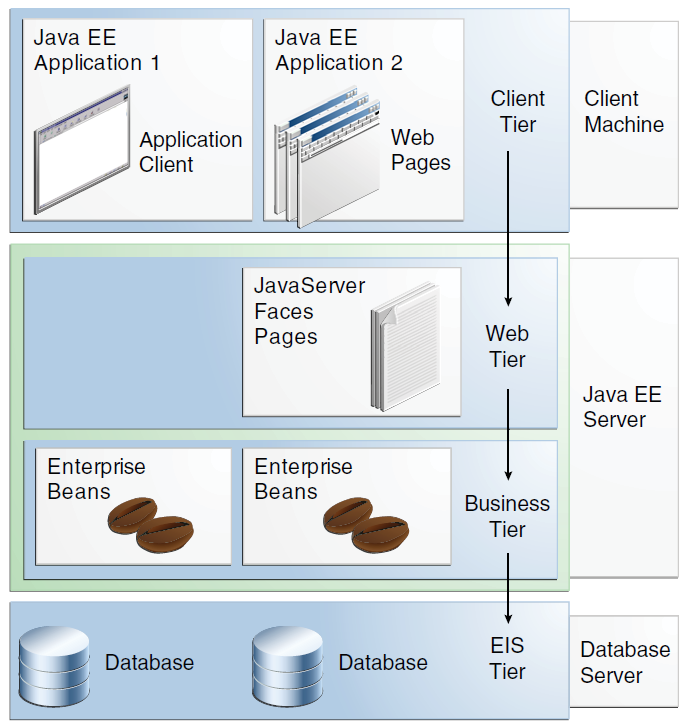
\includegraphics[width=\linewidth]{./images/jeearch}
\caption[jee arch]{JEE architecture}
\label{fig:jeearch}
\end{figure}

\clearpage

\subsection{Component View}\label{componentview}
\subsubsection{Database}
The persistence layer must include a DBMS component, in order to manage the insertion, modification, deletion of data and managing the relative transactions on the database.\\
Regardless of the implementation, the DBMS must guarantee the correct functioning of concurrent transactions and the ACID properties; it also must be a relational DBMS, since the application needs in terms of data storage do not require a more complex structure than the simple one provided by the relational data structure.\\
The data layer must only be accessible through the Application Server via a dedicated interface. With respect to this, the Application Server must provide a persistence unit to handle the dynamic behaviour of all of the persistent application data.\\
Sensible data such as passwords and personal information must be encrypted properly before being stored. Users must be granted access only upon provision of correct and valid credentials.\\
The E-R diagram illustrates a detailed view over the database schemas and attributes.

\begin{figure}[H]
\begin{center}
		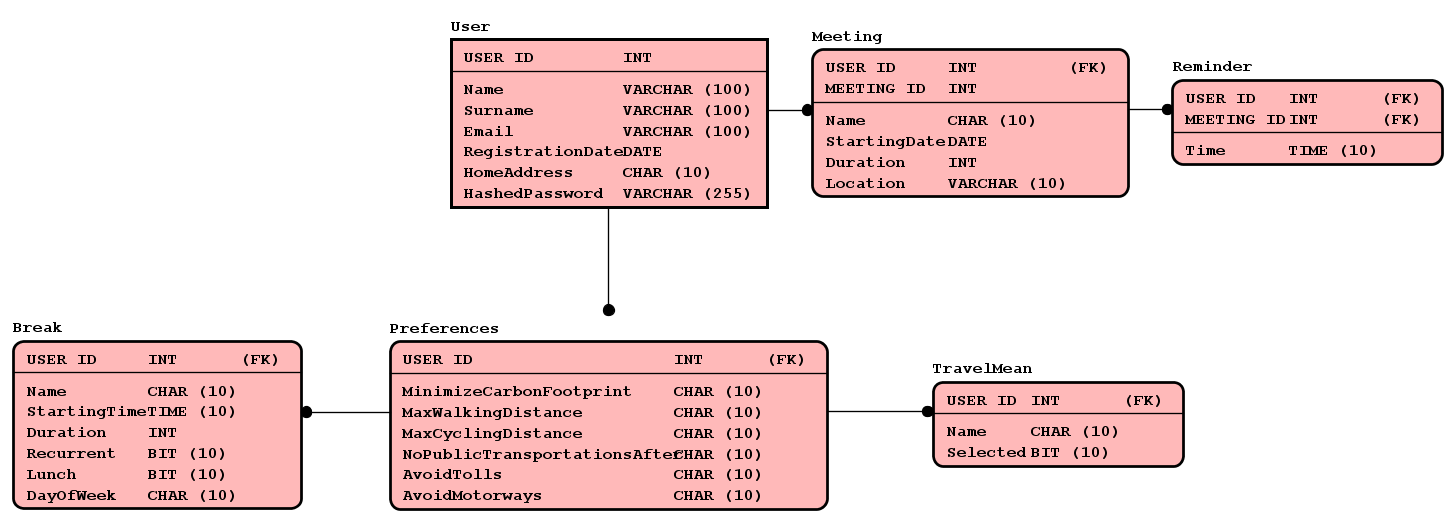
\includegraphics[width=1.3\textwidth]{images/ertravlendar}
		\caption{The E-R diagram of the database schema.}
		\label{erdiagram}
\end{center}
\end{figure}

\clearpage
We also provide a projection of the E-R diagram in the form of a class diagram:

\begin{figure}[H]
\begin{center}
		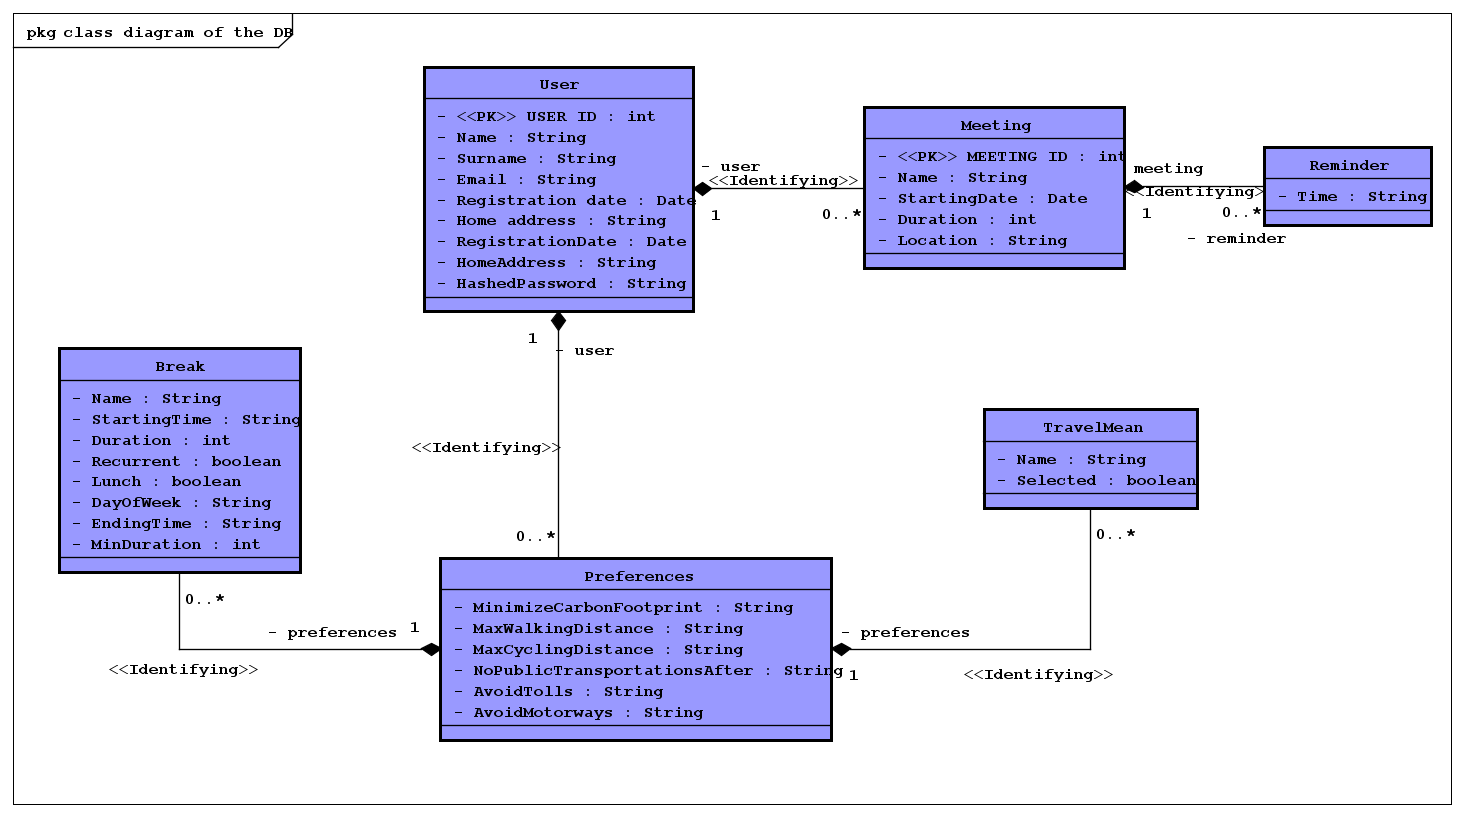
\includegraphics[width=1.3\textwidth]{images/databasedesignclass}
		\caption{The E-R diagram of the database schema.}
		\label{erdiagram}
\end{center}
\end{figure}



\clearpage
\subsubsection{High-level component diagram}
\begin{figure}
	\centering
	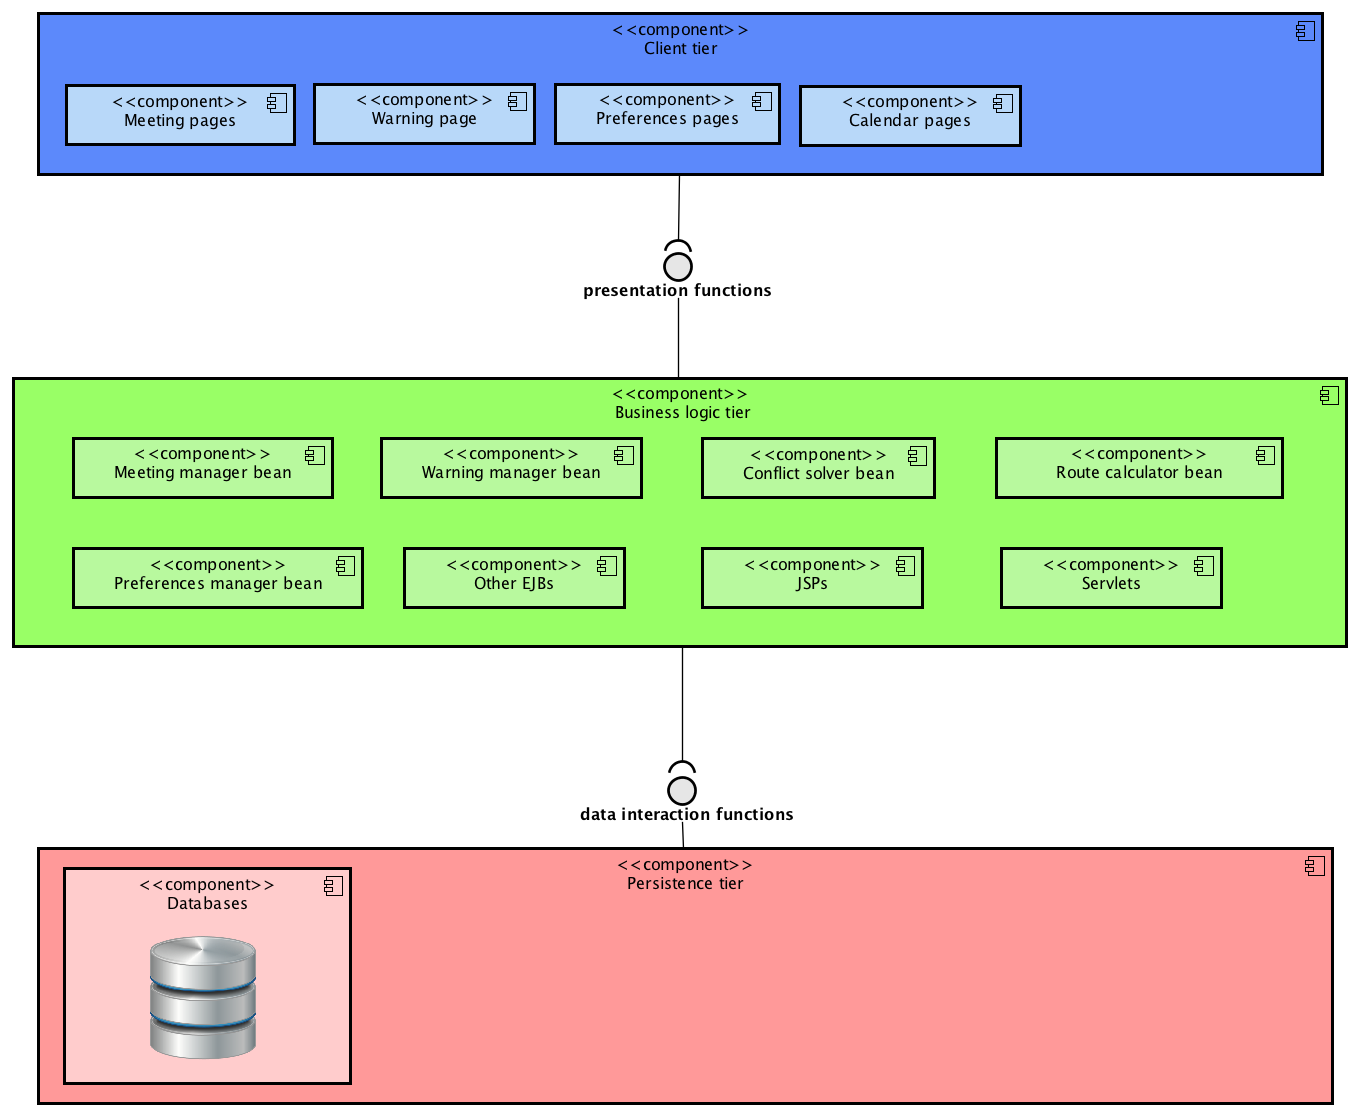
\includegraphics{Users/matteo/MarzialiMantovani/DD/images/HLcomponentdiagram}
	\caption[High-level component diagram]{}
	\caption{}
	\label{fig:hlcomponentdiagram}
\end{figure}

\clearpage
\subsubsection{Low-level component diagram}



\begin{figure} 
\begin{center}

\makebox[\textwidth]{%
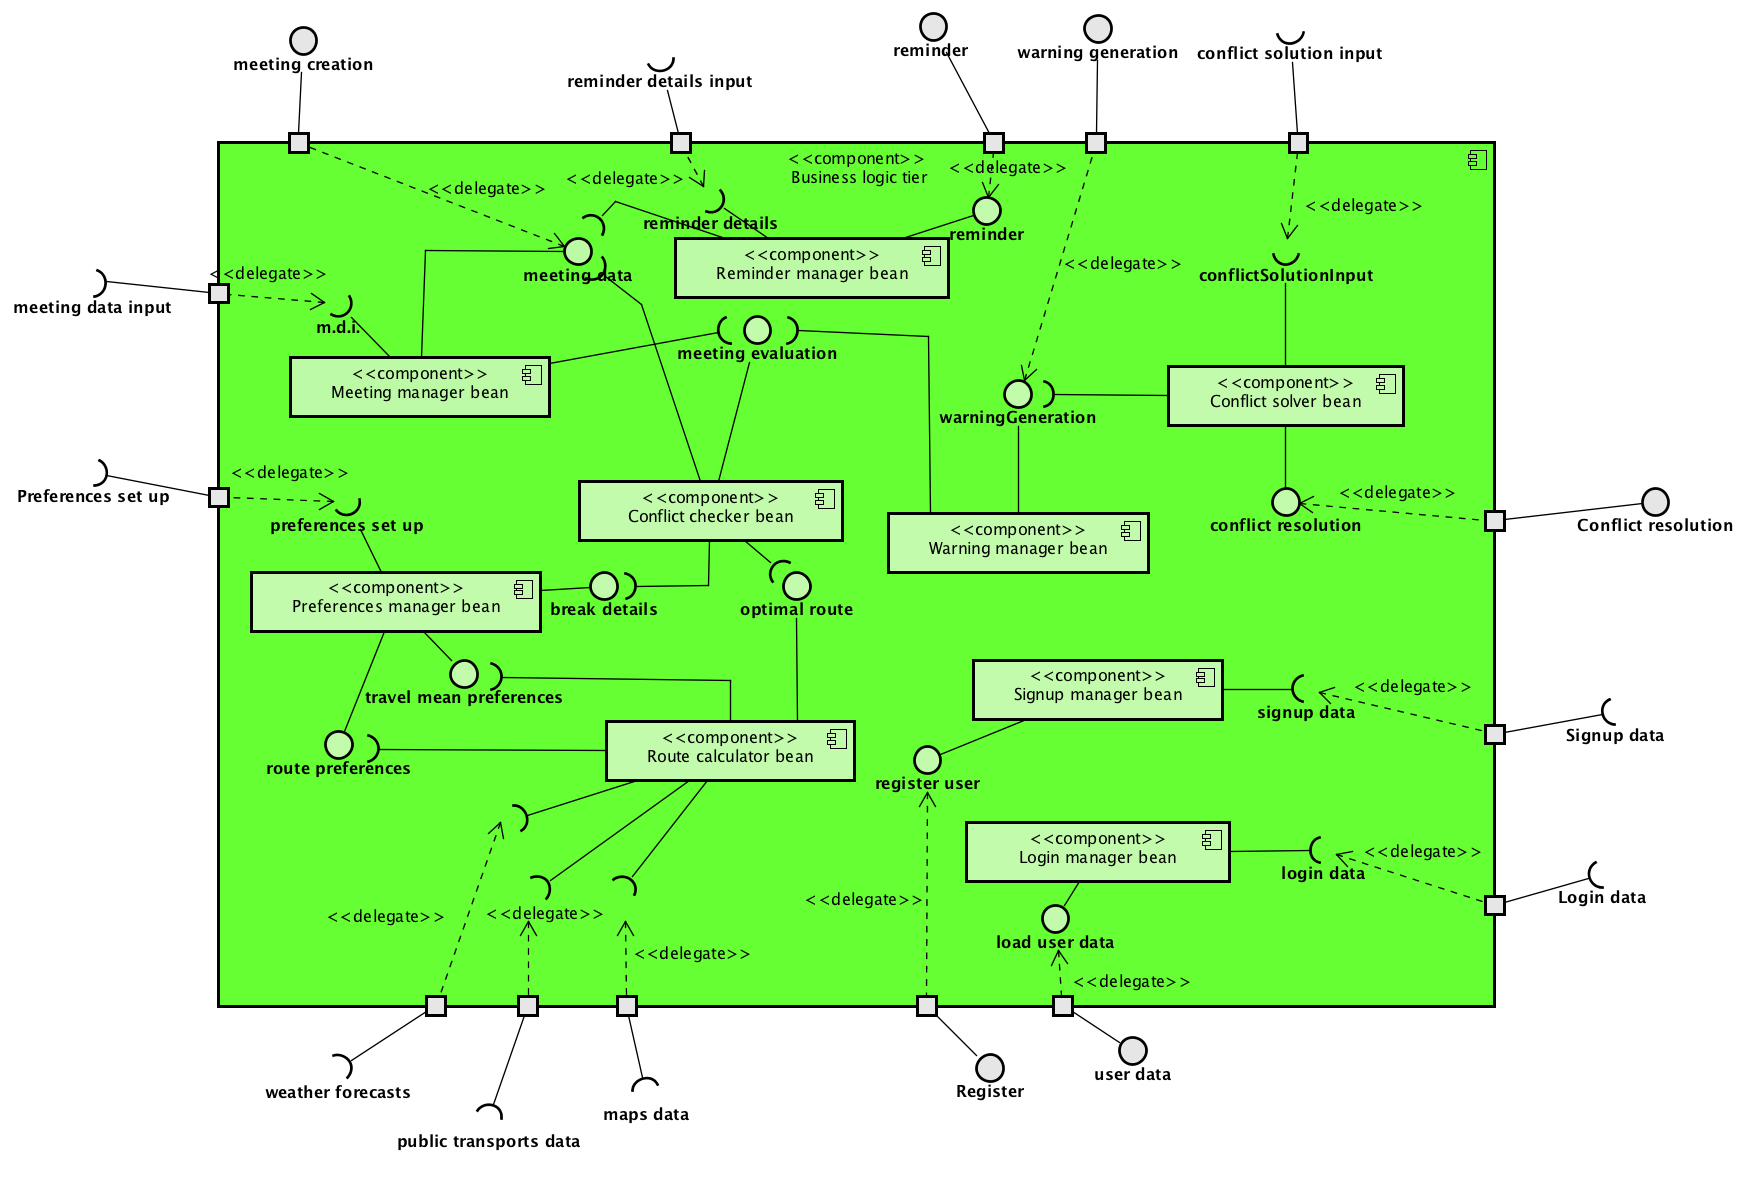
\includegraphics[width=1.5\linewidth]{images/LLcomponentdiagram} 
}
\caption{Low-level component diagram} 
\label{fig:llcomponentdiagram} 


\end{center}
\end{figure} 

\clearpage
\begin{flushleft}

\begin{table}[htp]

\begin{tabular}{l|p{7cm}}
 Component&analysis\\
\hline
\hline
Name&Meeting manager bean\\
\hline
Input interfaces&
	\begin{itemize}
	\item Meeting data input.
	\item Meeting evaluation.
	\end{itemize}
\\
\hline
Output interfaces& Meeting details 
\\
\hline
Description&This is the component responsible for managing the insertion of meeting data by the user, it also provides these details to the meeting evaluator bean and to conflict evaluator bean.
\\
\hline


\end{tabular}

\caption{Meeting manager  table } 
\label{tab:meetingmanagertable}

\end{table}

\end{flushleft}

\begin{flushleft}
	
	\begin{table}[htp]
		
		\begin{tabular}{l|p{7cm}}
			Component&analysis\\
			\hline
			\hline
			Name&Conflict checker bean\\
			\hline
			Input interfaces&
			\begin{itemize}
				\item Meeting data  \item Break details \item Optimal route.
			\end{itemize}
			\\
			\hline
			Output interfaces& Meeting evaluation\\
			\hline
			Description&The Conflict checker bean has the role to evaluate if a meeting can be scheduled with respect to the adjacent meetings and the breaks. To execute this critical computation it needs information about the breaks, the new meeting and the time to reach the meetings which precede and follow it. The result of the conflict checker bean is required by the conflict evaluator to establish whether it is necessary to generate a conflict or not. \\
			\hline
			
			
		\end{tabular}
		
		\caption{Conflict checker  table } 
		\label{tab:conflictcheckertable}
		
	\end{table}
	
\end{flushleft}

\begin{flushleft}
	
	\begin{table}[htp]
		
		\begin{tabular}{l|p{7cm}}
			Component&analysis\\
			\hline
			\hline
			Name&Warning manager bean\\
			\hline
			Input interfaces& Meeting evaluation\\
			\hline
			Output interfaces& Warning generation\\
			\hline
			Description&This component represents the bean which is responsible to generate a warning and submit it to the user if the meeting evaluator notify a conflict. \\
			\hline
				
		\end{tabular}
		
		\caption{Warning manager table } 
		\label{tab:warningmanagertable}
		
	\end{table}
	
\end{flushleft}

\begin{flushleft}
	
	\begin{table}[htp]
		
		\begin{tabular}{l|p{7cm}}
			Component&analysis\\
			\hline
			\hline
			Name&Conflict solver bean\\
			\hline
			Input interfaces& Warning generation\\
			\hline
			Output interfaces& Conflict resolution\\
			\hline
			Description&The conflict solver is the component that manages the resolution of conflicts, thus it is called by a new warning and his functions are to ask the user whether ignore or modify the meetings involved in a conflict and to apply his choice. \\
			\hline
			
		\end{tabular}
		
		\caption{Conflict solver table } 
		\label{tab:conflictsolvertable}
		
	\end{table}
	
\end{flushleft}

\begin{flushleft}
	
	\begin{table}[htp]
		
		\begin{tabular}{l|p{7cm}}
			Component&analysis\\
			\hline
			\hline
			Name&Preferences manager bean\\
			\hline
			Input interfaces& Preferences set up \\
			\hline
			Output interfaces&
			\begin{itemize}
					 \item Route preferences \item Travel mean preferences \item Break details
			\end{itemize}
			\\
			\hline
			Description&This is the component designed to assolve all the functions related to the preferences. Hence, it manages the insertion, update and deletion of the preferences about routes, travel means and breaks, furthermore it provides preferences details to other components when it is necessary. \\
			\hline
			
		\end{tabular}
		
		\caption{Preferences manager table } 
		\label{tab:preferencesmanagertable}
		
	\end{table}
	
\end{flushleft}

\begin{flushleft}
	
	\begin{table}[htp]
		
		\begin{tabular}{l|p{7cm}}
			Component&analysis\\
			\hline
			\hline
			Name&Route calculator bean\\
			\hline
			Input interfaces& 
			\begin{itemize}
				\item Travel mean preferences \item Route preferences \item Weather forecasts \item Public transport data \item Maps data
			\end{itemize} \\
			\hline
			Output interfaces& Optimal route\\
			\hline
			Description&This is the component designed to assolve all the functions related to the preferences. Hence, it manages the insertion, update and deletion of the preferences about routes, travel means and breaks, furthermore it provides preferences details to other components when it is necessary. \\
			\hline
			
		\end{tabular}
		
		\caption{Route calculator table } 
		\label{tab:routecalculatortable}
		
	\end{table}
	
\end{flushleft}

\begin{flushleft}
	
	\begin{table}[htp]
		
		\begin{tabular}{l|p{7cm}}
			Component&analysis\\
			\hline
			\hline
			Name&Signup manager bean\\
			\hline
			Input interfaces& Signup data \\
			\hline
			Output interfaces& Registration\\
			\hline
			Description&This is the component which manages the user signup process, from the insertion of personal data, through their storage on the database, to the account verification. \\
			\hline
			
		\end{tabular}
		
		\caption{Signup manager table } 
		\label{tab:signupmanagertable}
		
	\end{table}
	
\end{flushleft}

\begin{flushleft}
	
	\begin{table}[htp]
		
		\begin{tabular}{l|p{7cm}}
			Component&analysis\\
			\hline
			\hline
			Name&Login manager bean\\
			\hline
			Input interfaces& Login data \\
			\hline
			Output interfaces& User data \\
			\hline
			Description&This is the component dedicated to all the login steps. When the user insert in the apposite area his name and password, this component takes the data and provides the computations needed to verify the credentials and load the user's content. \\
			\hline
			
		\end{tabular}
		
		\caption{Login manager table } 
		\label{tab:loginmanagertable}
		
	\end{table}
	
\end{flushleft}


\clearpage
\subsection{Deployment View}\label{deploymentview}
The deployment diagram represent our intention to express a complete view of the system in terms of adopted hardware components, communication languages and  software components distribution among them. \\
Among the huge number of services, we have decided to use GlassFish as web and application server and to adopt the MySQL database management system. \\
As far as the software components are concerned, the application server has the Entity Java Beans and the Java Persistence API to allow the interaction with the database, oppositely the web server has the servlets and both the Java Server Pages and Faces because we still do not know which is the best component to develop among JSP and JSF.\\
Since we have initially thought about a mobile application, the web server could be omitted, however we have decided to insert it in our architecture to make the system ready to future improvements. \\ 
The diagram is filled with a grey box named 'External services servers' to design also the interaction between our system and the systems of other institutions such as Google Maps or the municipality of Milan etc. which can provide basical data to reach our goals and to implement Travlendar+ functions.\\


\begin{figure}
	\centering
	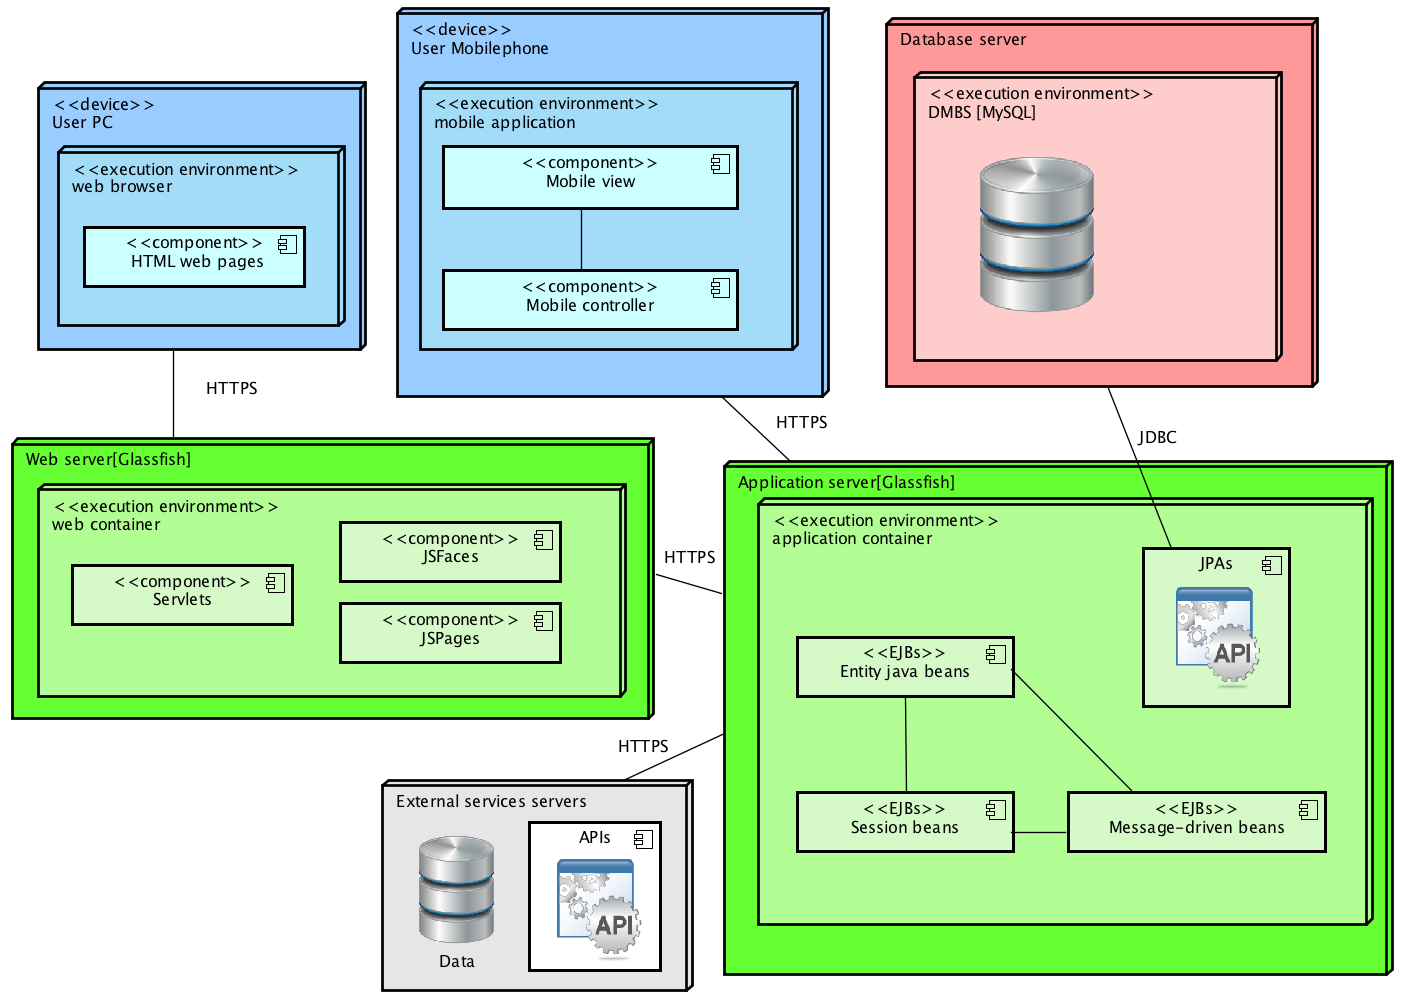
\includegraphics[width=1.3\textwidth]{images/deploymentdiagram}
	\caption{Deployment diagram}
	
	\label{fig:deploymentdiagram}
\end{figure}
\begin{figure} 
\begin{center}

\makebox[\textwidth]{%
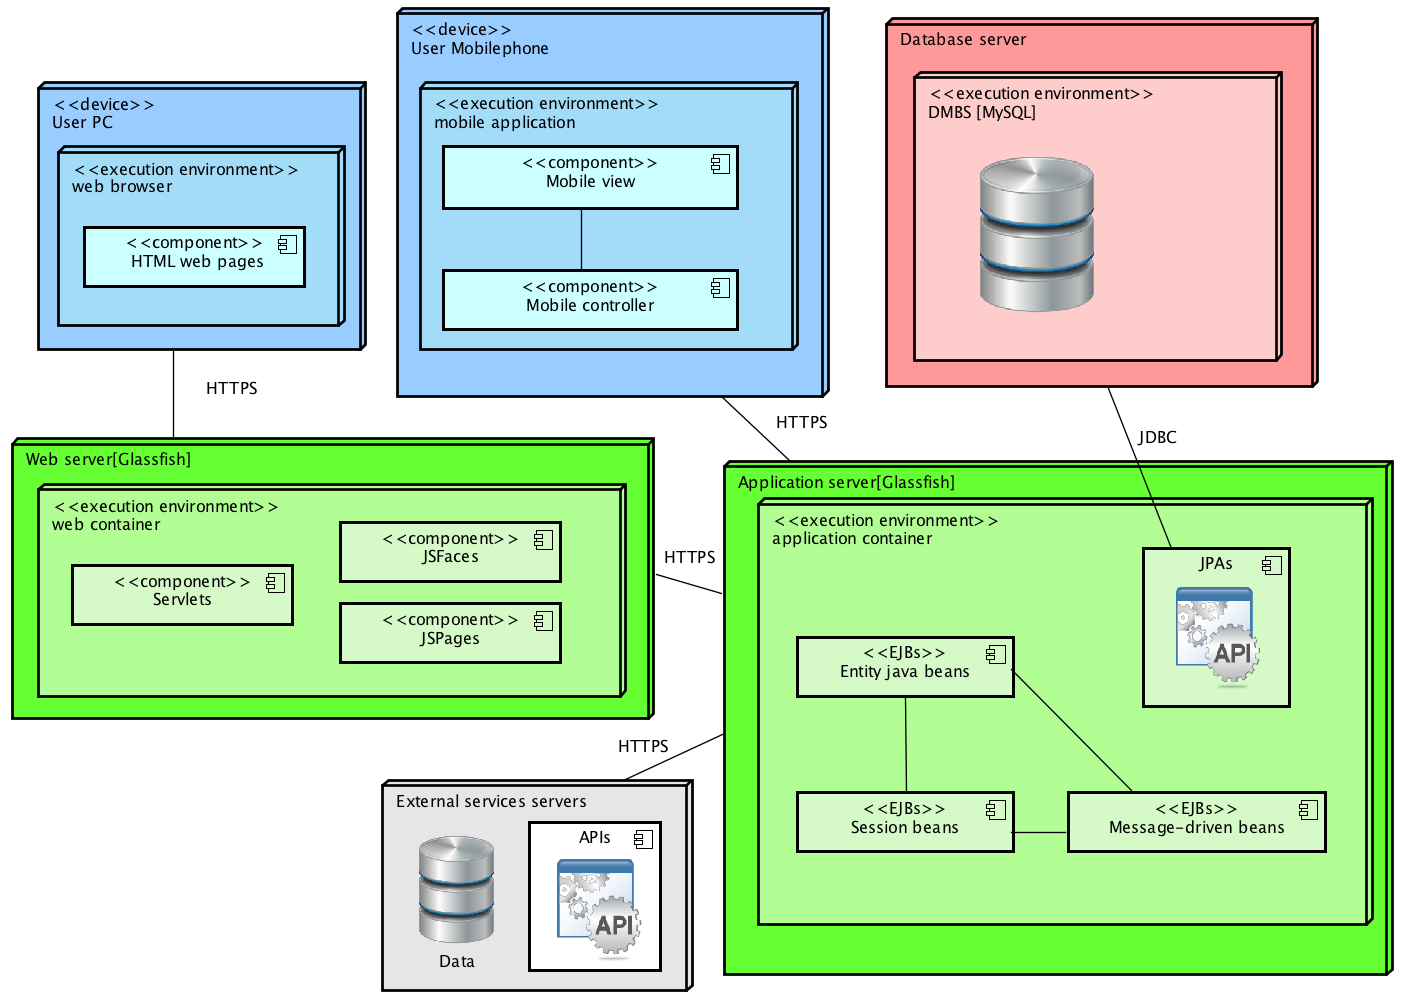
\includegraphics[width=1.5\linewidth]{images/deploymentdiagram} 
}
\caption{Deployment diagram} 
\label{fig:deploymentdiagram} 


\end{center}
\end{figure} 
\clearpage

\subsection{Runtime View}\label{runtimeview}
\subsubsection{Signup/login sequence diagram}
\begin{figure}
	\centering
	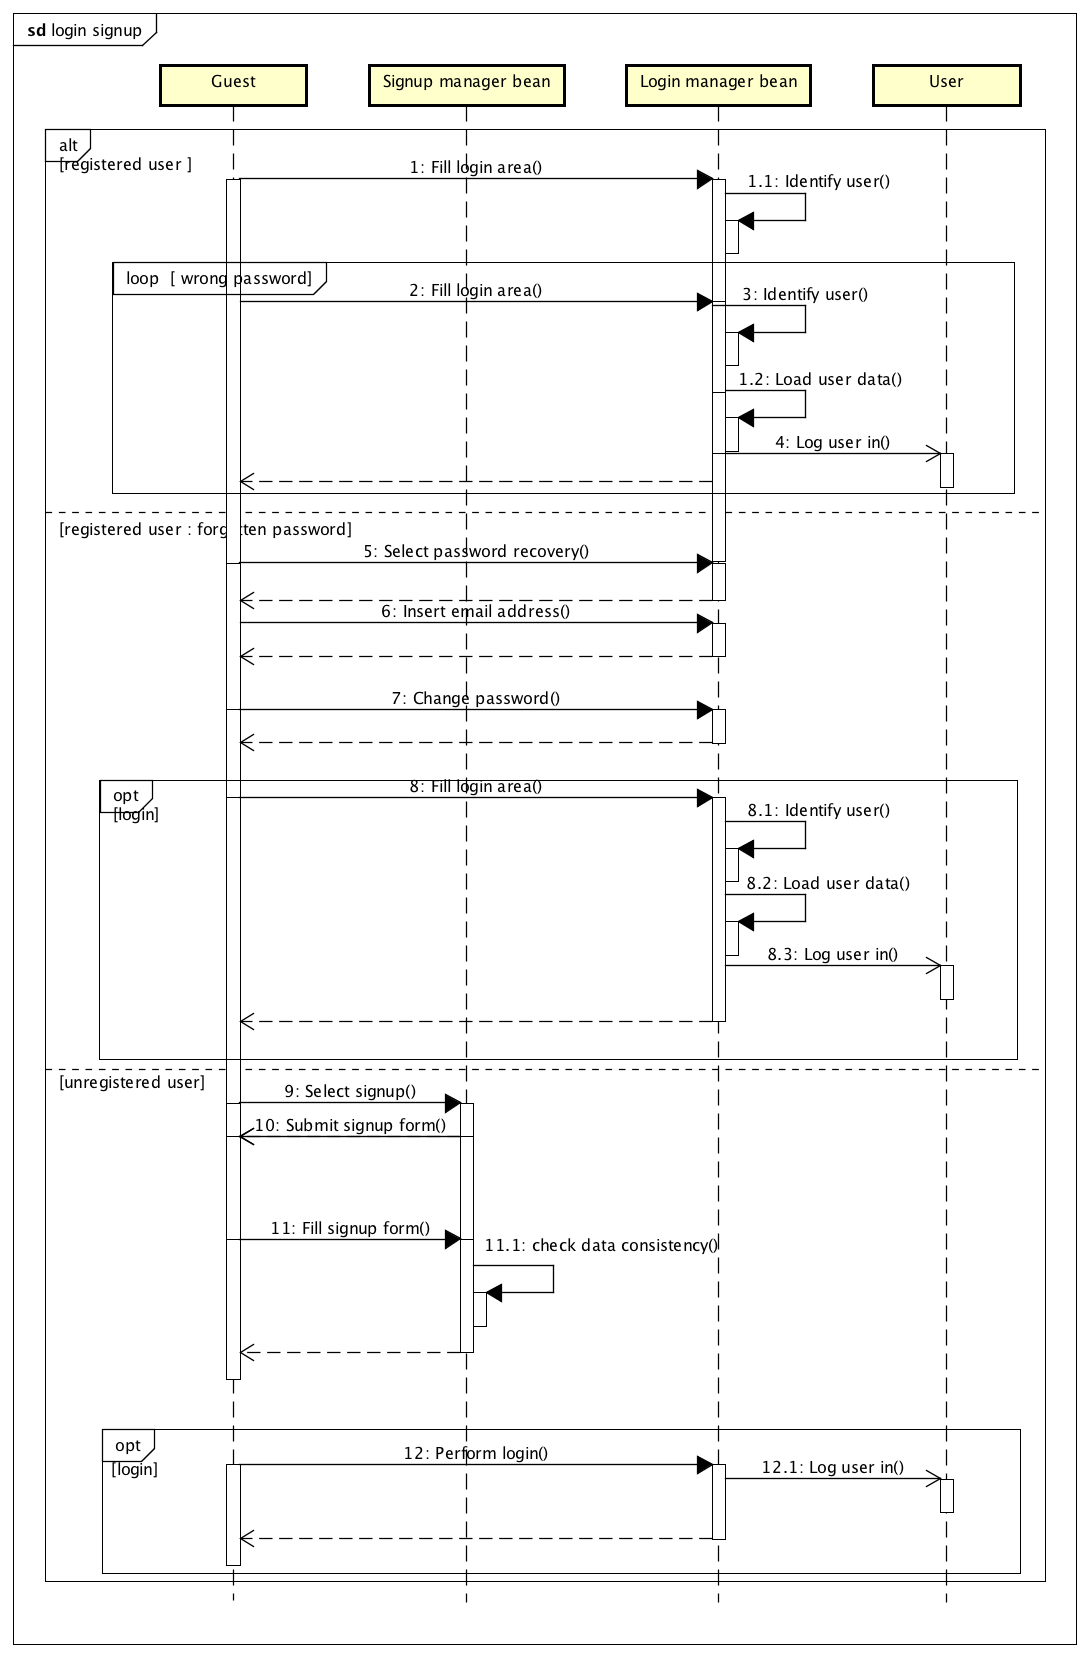
\includegraphics[width=1.3\linewidth, height=0.8\textheight]{images/signuplogin.png}
	\caption{Signup/login sequence diagram}
	
	\label{fig:signuplogin}
\end{figure}


The Signup and Login runtime view includes, as the name suggests, both the signup and the login (and also the password recovery), since they are intended related concepts with a slight impact on the application behaviour. \\
A registered user who wants to log in himself must fill the login form until he insert correctly his username and password, at this point the Login manager bean manages to identify him and then to load his data. \\
On the other hand, when an unregistered user shows the intention to sign up himself, the Signup manager bean is called and submits the user a registration form, and, once the user has completed and sent back it, manages to verify the consistency of the inserted data. \\ 
If a registered user has forgotten his password, the Login manager component is called and requires the user email to send him a link where a new email can be created, then the login can eventually be performed by the user. \\

\clearpage
\subsubsection{Meeting creation sequence diagram}
\begin{table}[htp]

\begin{tabular}{r|p{7cm}}
\bf\large Name&\bf\large Creation of a meeting\\
\hline
\hline
\bf Actors&User\\
\hline
\bf Entry conditions&The user is logged in and is in the main page.\\
\hline
\bf Flow of events&
\begin{itemize}

\item The user clicks on "Create meeting" button and he is redirected to the page with the input form to create a meeting.

\item The user fills up the form with the meeting information (title, location, description, date and time, flags, etc...).

\item The system checks whether the meeting at the specified time and date is possible according to the user preferences and the current daily schedule, the optimal route is proposed.


\item The user is then redirected to the main page.

\end{itemize}
\\
\hline
\bf Exit conditions&The new meeting with the calculated optimal route is added to the user Calendar. In the case of the incompatibility of a meeting with others a warning is created.\\
\hline
\bf Exceptions&The information inserted is wrong or some information is missing: a corresponding error is displayed and the user is asked to modify the inserted information accordingly.
\\
\hline

\end{tabular}
\caption{Meeting Creation Use Case table}
 \label{tab:meetingcreationtab}
\end{table}
The meeting creation runtime view, explained through an apposite sequence diagram, summarize all the computations needed to allow the creation of a meeting. \\
This scenario starts when a user select to create a meeting, this intention is dispatched by the application server to the Meeting manager bean, which is in charge of submitting a meeting creation form to the user and holding its resubmission. \\
Taken the meeting details, the Meeting manager sends them to the conflict checker, this component must control whether a meeting is feasible or not, considering both the breaks set by the user and other meetings. \\
To assolve this function, this bean needs thee break details from the preferences manager bean and some routes from the google maps server in order to evaluate the time among adjacent meetings. \\
Collected the information, the conflict checker computes to find overlaps and if it is not the case, the negative verification outcome reaches the user, who is notified about the correct insertion. In case overlaps are present, if they are caused by conflicts with breaks that can be flexibly rescheduled during their range not to be overlapping the meeting will be accepted without any consequence. Otherwise, if either this is not the case or the conflict is beetween meetings, the conflict checker will generate a conflict and notify the user through the meeting manager. 
\clearpage
\subsubsection{Conflict management sequence diagram}


\begin{figure} 
\begin{center}

\makebox[\textwidth]{%
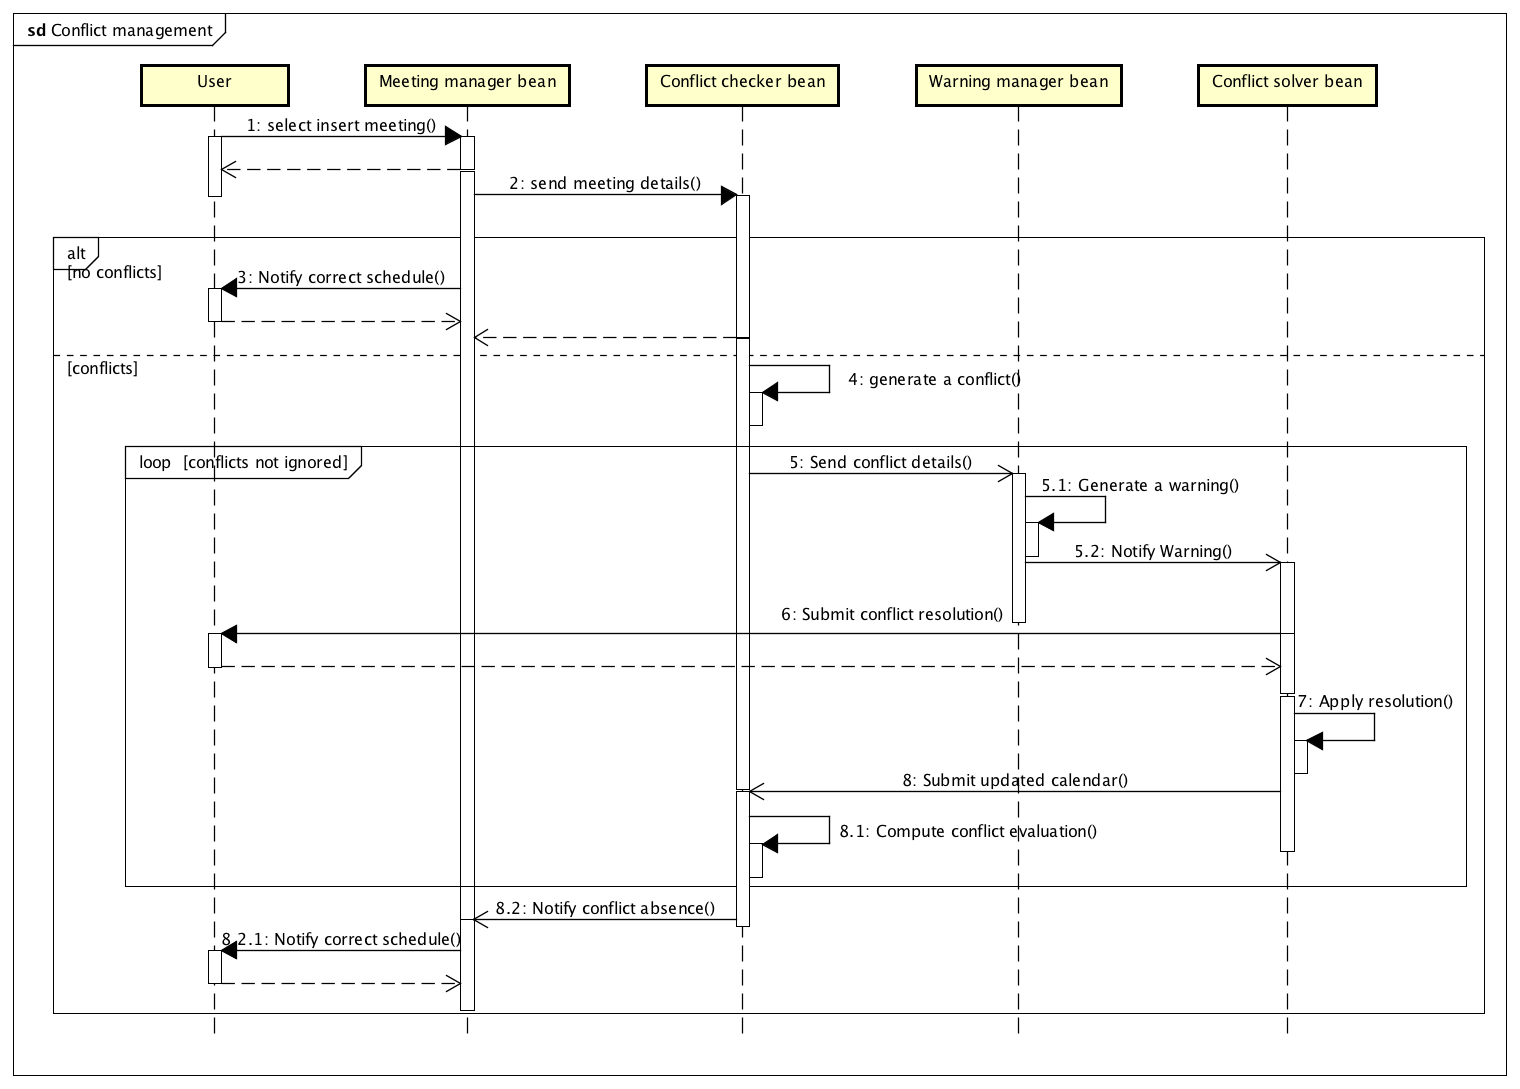
\includegraphics[width=1.7\linewidth]{images/conflictmanagement} 
}
\caption{Conflict management sequence diagram} 
\label{fig:conflictmanagement} 


\end{center}
\end{figure} 
The conflict management runtime view refers to every situation in which a conflict is generated even if in the provided sequence diagrams the computations start with a meeting insertion. We have already discussed the positive outcome that simply ends with a notification to the user, now we want to deeply analyze the presence and the management of a conflict. \\
When a conflict is found, the conflict checker notifies the warning manager which generates a warning in the system and notifies the conflict solver component, that is in charge of asking the user in which way he/she intend to solve the conflict and is in charge of applying the user choice. \\
Firstly, the conflict solver manages to ask the user whether ignore the conflict or modify the involved meetings to solve it. Then, it holds the user decision and computes to make it effective in the system. \\
If the conflict is ignored, it is deleted and the system behaves like it isn't any conflict. Otherwise, if the conflict is solved by the user, the conflict solver sends an updated calendar to the meeting evaluator which computes to verify overlaps. \\
If conflicts are found this cycle of operations is repeated, else the user is notified that his schedule is consistent. \\


\clearpage
\subsubsection{Break creation sequence diagram}


\begin{figure} 
\begin{center}

\makebox[\textwidth]{%
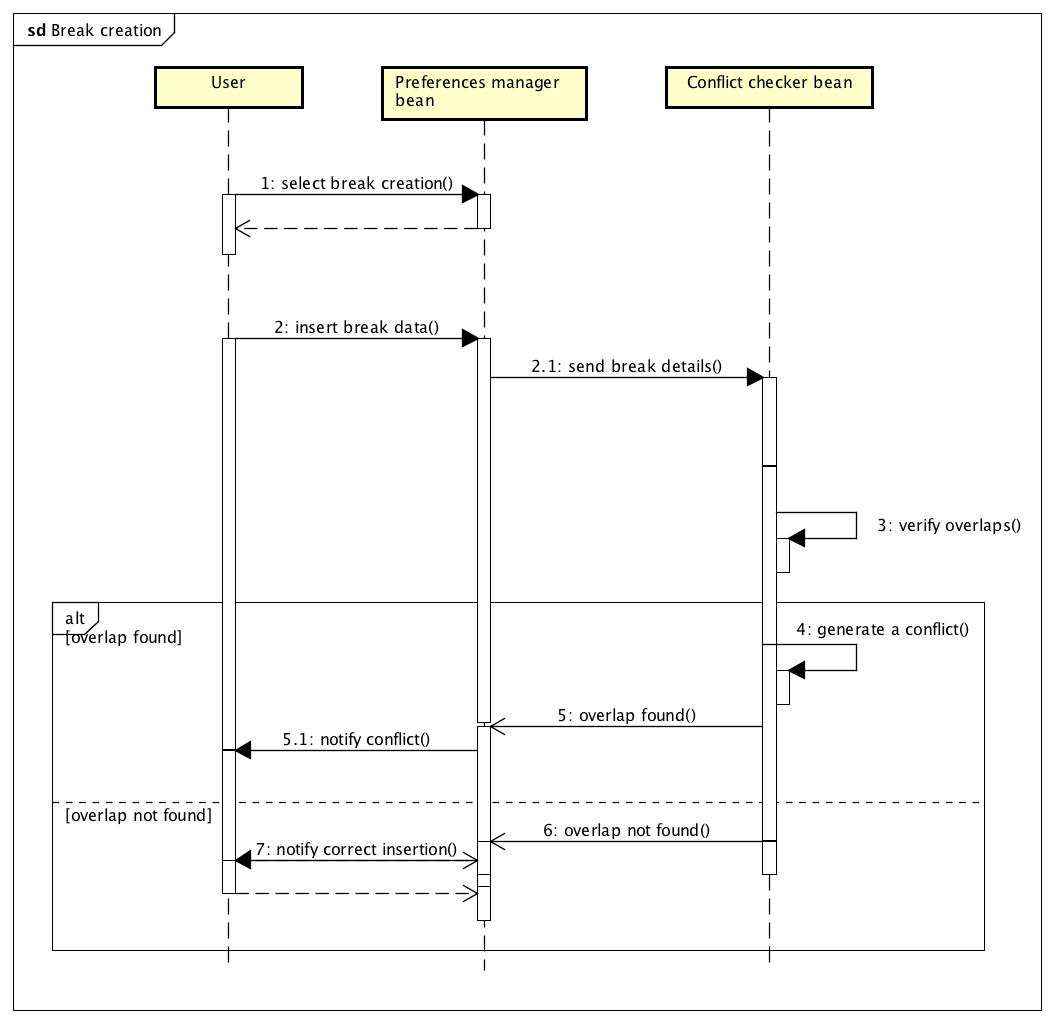
\includegraphics[width=1.7\linewidth]{images/breakcreation} 
}
\caption{Break creation sequence diagram} 
\label{fig:breakcreation} 


\end{center}
\end{figure} 
The break insertion runtime view is conceptually similar to the meeting insertion even if it involves less components and requires less controls. \\
When the user express the intention to insert a break, the preferences manager bean is called and manages to submit the user a form to get the break details. At this point, the preferences manager sends this details to the meeting evaluator which plays the role to search conflicts by verifying overlaps.\\ If it finds conflicts, it generates a conflict in the system otherwise nothing is done and in both cases the user is notified. \\ Please note that in the break insertion the only possible conflict refers to a situation where the new break overlaps completely one or more meetings which has the only implication of generating a conflict in the system. \\
\clearpage
\subsubsection{Preferences set up sequence diagram}
\begin{figure}
	\centering
	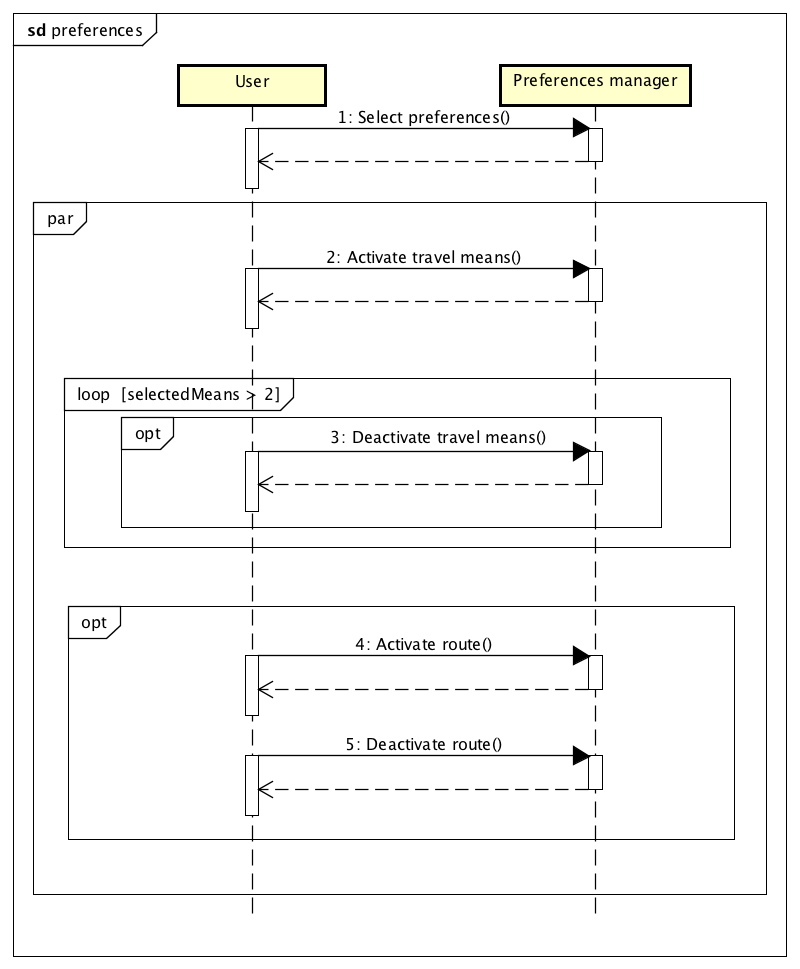
\includegraphics[width=1.3\textwidth]{images/preferences}
	\caption{Preferences set up sequence diagram}

	\label{fig:preferences}
\end{figure}

The preferences insertion runtime view aims to provide a representation of how a user can set up all the customizable settings of Travlendar+.\\ 
Firstly, it is relevant to notice that the breaks preferences are considered in a different sequence diagram. \\ 
This said, the user still can activate or deactivate travel means, to allow or prevent them to be used in the routes for his meetings, clearly at least one travel mean must be activated, this explains the travel means deactivation loop and its condition. \\
Moreover a user can eventually activate or deactivate routes, in the sense that a user can decide to have the fastest route, the shortest route etc. As far as the routes are concerned, there arenn't constraints referring to have at least one route activated, indeed in that case it is expected that a default route is adopted. 
\clearpage

\subsection{Component Interfaces}\label{componentinterfaces}
This sections includes further details on the interfaces between different macrocomponents and components of the system. Also, Subsection \ref{internalinterfaces} is devoted to illustrate some relevant details about the interfaces needed to use and interact with each component of the Application Server, accessible both by other Application Server components and by other components of the system.

\subsection{Database - Application Server}
The Application Server is the only one that can access the Database directly; this is done through the Java Persistence API mapping between objects and actual relations.

\subsection{Web Server - Web Browsers}
The interactions between the client's browsers and the Web Servers are based on the HTTPS protocol, with standards GET and POST methods.

\subsection{Application Server - Web Server and Clients}
The communication between Application Server and clients happen with the HTTP.

\subsection{Application Server - External Systems}
The Application Server must interact with external APIs like the Google Maps one, which will provide information about travels.

\subsection{Selected architectural styles and patterns}\label{archstyles}
\subsubsection{MVC Pattern}
Model-View-Controller pattern divides a given software application into three interconnected parts, so as to separate internal representations of information from the ways that information is presented to or accepted from the user. This is one of the most common and effective ways to avoid a dangerous level of coupling between the various parts of the whole system.

\subsubsection{4-tier Architecture}
A standard JEE 4-tier architecture was used to design the system, where the layers are, as better described in [Section \ref{higharch}] \textbf{High-Level components}:
\begin{itemize}
\item \textbf{Client Tier}
\item \textbf{Web Tier}
\item \textbf{Business Logic Tier} 
\item \textbf{Persistence Tier}
\end{itemize}

\subsubsection{Client-Server}
A client-server programming approach was used to design the application, in particular, the choice was to create a thin client, and makes all the logic and controlling reside in the Application server, which must have enough computing power to manage concurrent accesses in an efficient way.
On the other hand, the mobile application is only in charge of the presentation and it does not involve decision logic.

\subsubsection{Deployment}
\begin{itemize}
\item \textbf{Divide et impera:} software is divided in 4 independent tiers that put together offer the Travlendar+ application services.
\item \textbf{Cohesion:} each module has his specific purpose; Client tier handles the system clients; Logic tier handles the application processing and the Data layer that handles and manages the persistence of data.
\item \textbf{Decoupling:} the sofware components are independent and communicates through interfaces 
\item \textbf{Flexibility:} implied from decoupling, abstraction and reusability properties.
\item \textbf{Anticipating obsolescence:} if the technologies that compose a tier become obsolete, a tier can be substituted without affecting the others.
\item \textbf{Portability:} each tier can be run on different platforms.
\end{itemize}



\subsubsection{Structure style}
An Object-Oriented Architectural Style was chosen. It supports the division of responsibilities for a complex system into small and reusable parts called "Objects".
\\They communicate with each other through interfaces, by sending and receiving messages or by calling methods on other objects. 
The main benefits are: 
\begin{itemize}
\item \textbf{Extensibility:} change of implementation does not imply an interface change
\item \textbf{Reusability:} objects are developed as small reusable piece of software 
\item \textbf{Testability:} encapsulation improves testability

\end{itemize}  



\subsection{Other design decisions}\label{otherdecisions}

\clearpage
\section{Algorithm Design}
\subsection{Meeting Warning checker algorithm}

One of the fundamental identified algorithms is the one that checks whether a newly added meeting can generate a warning with the previous meeting, the following, or both of them.
If it's one of those cases a warning containing the correct meetings is created in the system (see createWarning method in the code).
\\
The pseudocode of the algorithm is provided below:
\\

\lstinputlisting[language=pseudocode]{subsections/warningpseudocode.txt}

\subsection{Break Warning checked algorithm}

Another important algorithm is the one that checks whether a newly added meeting can generate a warning with one or more breaks, this is a little bit more complicated because in the most general case no one forbids a user to insert overlappings breaks, more meetings entirely within the limits of a single break or even nested breaks.
\\The proposed algorithm will be able to handle all the various cases. What has not yet taken into consideration is that if a meeting is in conflict with a break, this does not necessarily mean that the only way to solve this conflict is to modify THIS precise meeting that was discovered as problematic, another possibility could be to shift other meetings happening in the break limits range in order to make space for the minimum duration of the break to fit in.
\\
The pseudocode of the algorithm is provided below:
\\

\lstinputlisting[language=pseudocode]{subsections/breakpseudocode.txt}



\section{User Interface Design}
\subsection{UX Diagram}
As a way to show the navigation among the different pages and define the visual flow of screens we designed a User Experience diagram.


TODO 




\subsection{Mockups of the User Interface}
	\begin{flushleft}
		Concerning the user interface requirements, we established to directly provide information about the application screens and layout through several mockups. \\
		We designed the sketch of the main pages of Travlendar+ following our aim to make a light and user friendly product but, at the same time, we have pursued an attractive and impressive style. \\
		Apparently, the coding phase could affect our desing. Hence, these sketches are not definitive, their aim is to give an idea of the application design. \\
		For this reason, if we notice that some changes are necessary due to either app. improvement or obstacles in realization, we would be ready to modify them. 
	\end{flushleft}
\clearpage

	\begin{figure}
			\begin{flushleft}
			\subsubsection{Homepage}
			To pursue our aim of realizing a user-friendly and light app, we decided to provide the main functions directly in the homepage. Indeed, from this page, a guest can reach the sign up form, a user can log himself in,can insert a meeting by tapping onto a day in the calendar,can manage his preferences and even access the warnings. \\ 
		\end{flushleft}
		\centering
		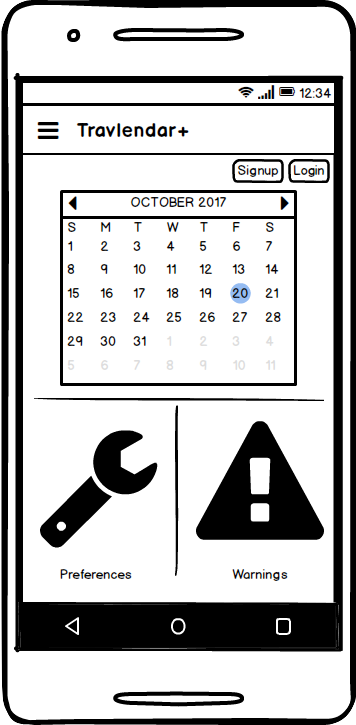
\includegraphics[width=0.6\linewidth]{mockups/Homepage}
		\caption{Travlendar+ homepage.  
		}
	\label{fig:homepage}
	\end{figure}

	\begin{figure}
			\begin{flushleft}
			\subsubsection{Quick Menu}
			We thought about a quick menu to collect some secondary functions, to make them easily reachable. By tapping on the top-left corner of the app people have the opportunity to either register or log in themselves, to only view meetings of the current day, to access the reminders they set up, to manage the warnings and to logout if they are already logged in.
		\end{flushleft}
	\centering
	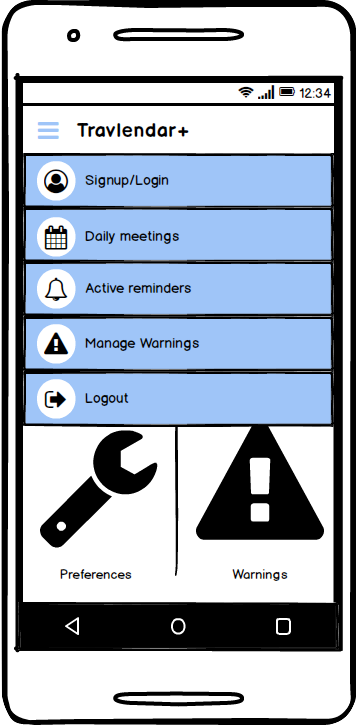
\includegraphics[width=0.6\linewidth]{mockups/QuickMenu}
	\caption{Quick access menu.}
	\label{fig:quickmenu}
	\end{figure}
\clearpage

	\begin{figure}
			\begin{flushleft}
			\subsubsection{Meeting Creation}
			This page is a very simple form, which allows the user to finalize the creation of a meeting by filling it in all its fields. 
			The house-logo in the  right corner,on the top band and near the application name, represents the return-to-homepage icon. 
		\end{flushleft}
		\centering
		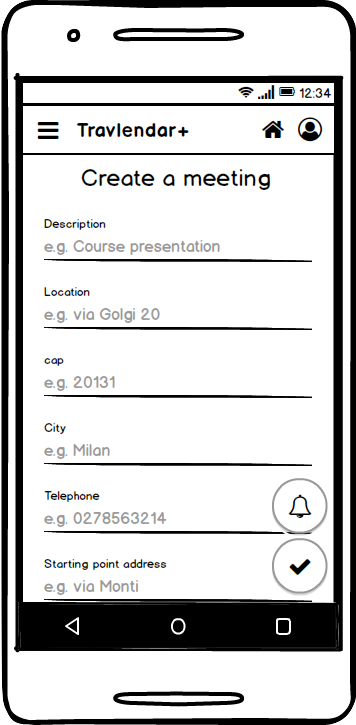
\includegraphics[width=0.6\linewidth]{mockups/CreateMeeting}
		\caption{Meeting creation page.}
		\label{fig:createmeeting}
	\end{figure}

	\begin{figure}
			\begin{flushleft}
			\subsubsection{Meeting Page}
			This screen wants to provide all the useful information related to a meeting already registered in the system. First details provided, in the highest portion of the page, regard the meeting location and the route to reach the appointment, further information are located below. In addition, on the right part of the screen, there are quick access buttons: the "plus" icon allows the user to add a reminder for the event, the "pencil" icon is to change meeting details and the "x" button provides deletion function. 
		\end{flushleft}
	\centering
	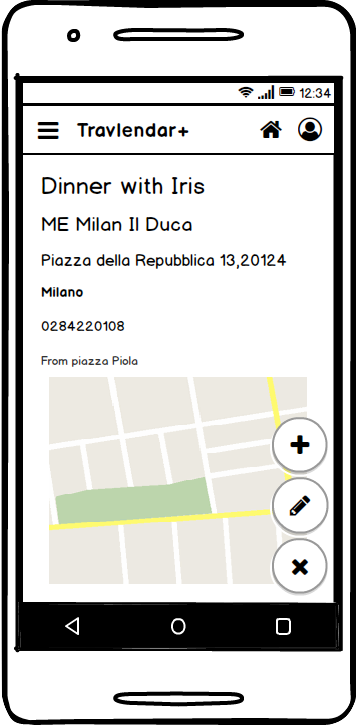
\includegraphics[width=0.6\linewidth]{mockups/MeetingView}
	\caption{Meeting view page. }
	\label{fig:meeting-view}
	\end{figure}
\clearpage

	\begin{figure}
			\begin{flushleft}
			\subsubsection{Warning Page}
			The warnings page has the role to summarize and notify all the conflicts among meetings which involve the user's appointments. Every warning is represented by a dialog which points out the meetings that generate the conflict and which has two buttons, one to ignore the warning and other one to solve it by modifying the conflictual meetings. 
			To prevent too much user's clicks, an "ignore all" button is provided, which is equivalent to tap "ignore" for each warning in the list. 
		\end{flushleft}
		\centering
		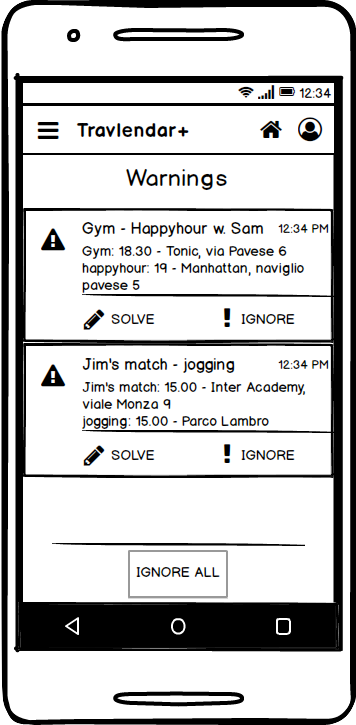
\includegraphics[width=0.6\linewidth]{mockups/Warnings}
		\caption{Warnings page}
		\label{fig:warnings}
	\end{figure}
\clearpage

	\begin{figure}
				\begin{flushleft}
				\subsubsection{Travel means preferences}
			This is a very simple page with a minimalistic design, not to uselessly load the application. However, this basical view provides all the functions which the user needs to select his preferences related to the transports for his travels. 
			Please notice that the preferences section can be changed by tapping on an specific topic just below the "Preferences" bar.
		\end{flushleft}
		\centering
		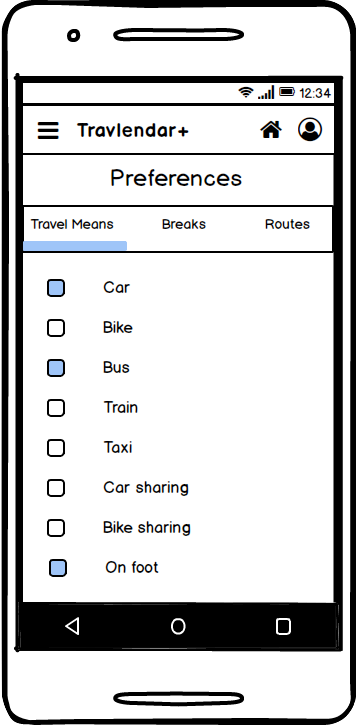
\includegraphics[width=0.6\linewidth]{mockups/PreferencesTravelMeans}
		\caption{Travel mean preferences page.}
		\label{fig:preferencestravelmeans}
	\end{figure}

		\begin{figure}
				\begin{flushleft}
				\subsubsection{Breaks preferences}
				The breaks page consists in a list of events, that represent pauses, organized in order of creation and labeled by the type of the break. For every break  both the starting and the ending time, a "pencil" button to allow modifications and a "x" button,to remove it, are provided. In addition, thanks to the fact that we decided to make the breaks general, that means not related to a specific day, the user has the faculty to either flag or unflag them to activate or deactivate them. 
			\end{flushleft}
		\centering
		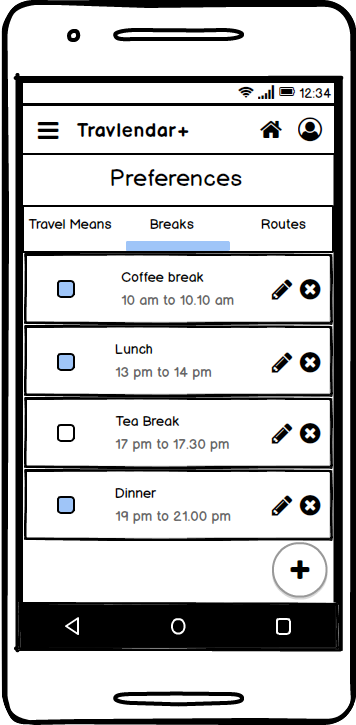
\includegraphics[width=0.6\linewidth]{mockups/PreferencesBreaks}
		\caption{Break preferences page.}
		\label{fig:preferencesbreaks}
	\end{figure}
	
		\begin{figure}
				\begin{flushleft}
				\subsubsection{Route preferences}
				The route preferences page is very similar to the Travel mean preferences page. The style is the same and the opportunity to flag or unflag elements too, however there are differences. Some of the preferences in this section are mutal exclusive, so the user is prevented to select more than one of them (for instance a user can select either the shortest route or the fastest). Moreover, some selection element has customizable details, they are represented with a pencil logo on the right, and can be managed by the user to best fit his preferences (for example the user can select after which hour he does not want to use public transportations).
			\end{flushleft}
		\centering
		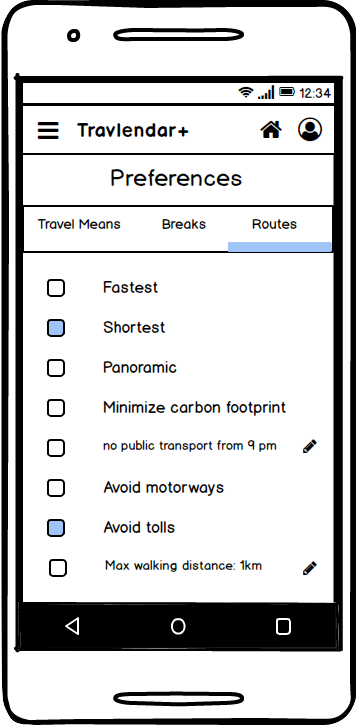
\includegraphics[width=0.5\linewidth]{mockups/PreferencesRoutes}
		\caption{Route preferences page}
		\label{fig:preferencesroutes}
		
	\end{figure}
	

\clearpage
\section{Requirements Traceability}
In order to have a simplified and schematic view over the designed components that are going to satisfy the requirements and provide the functionalities which were identified in the RASD document we define a formal mapping that explicitely correlates the Goals and functions with one or more Components that should be able to achieve the goal and create the functionality.

\begin{flushleft}

\begin{table}[htp]

\begin{tabular}{p{3cm}|p{6cm}|p{2cm}}
 Goal&Functions&Components\\

\hline
\hline
\textbf{[\hypertarget{G1}{G1}]}  Memorizing and organizing both events and appointments on the calendar. &\textbf{[\hypertarget{F2}{F2}] Meeting creation}: This is the most important function of the app, it allows to generate an event related to an appointment. It requires the user to define all the details such as date, time, location, starting point, preferences etc. & \autoref{tab:meetingmanagertable}\\
\hline
 \textbf{[\hypertarget{G2}{G2}]} Being sure to reach the appointment location in time avoiding delays. &
 \begin{itemize}
 	\item \textbf{[\hypertarget{F6}{F6}] Reminder management}: The applications allows users to set up reminders for a certain Meeting in order for the user not to be late for it.
 	
 	\item \textbf{[\hypertarget{F8}{F8}] Update meetings}: This function is both basic and relevant, it allows the user to customize his meetings after their creation. In other words, through this functionality the user can modify each one meeting details, even in case of a warning is generated.
 \end{itemize}
& 
\begin{itemize}
	\item \autoref{tab:routecalculatortable}
	
	\item \autoref{tab:meetingmanagertable}
\end{itemize}
\\
\hline
\textbf{[\hypertarget{G3}{G3}]} Being sure not to schedule overlapping meetings. &
\begin{itemize}
	\item \textbf{[\hypertarget{F9}{F9}] Warnings management}:  In case a warning is generated by the system due to a possible overlap among two or more meetings, the user must solve the warning. In other words, the user has to decide wheter he wants to ignore the overlap notification or he intend to modify some meetings to be sure that he can reach and participate to all his appointments.
	
	\item \textbf{[\hypertarget{F4}{F4}] Delays management}:  If the app had noticed, according to the estimated travel time, that the user is in late, and he previously had inserted the email address of the meeting’s participants, Travlendar+ would notify them about the delay. 
\end{itemize}&
\begin{itemize}
	\item \autoref{tab:conflictcheckertable}
	
	\item \autoref{tab:conflictsolvertable}
	
	\item \autoref{tab:warningmanagertable}
\end{itemize}\\
\hline


\end{tabular}
\caption{Traceability table } 
\label{tab:traceabilitytable1}
\end{table}

\begin{table}[htp]
	
\begin{tabular}{p{3cm}|p{6cm}|p{2cm}}
\hline
\textbf{[\hypertarget{G4}{G4}]} Being able to use only travel means that fit with user preferences. &\textbf{[\hypertarget{F3}{F3}] Preferences set up}: An important feature of Travlendar+ consists in allowing the user to filter out specific routes depending on some constraints about the travel, or to set break-dedicated time slots.&
\autoref{tab:preferencesmanagertable}\\
\hline
\textbf{[\hypertarget{G5}{G5}]} Preventing the user to forget an appointment.&\textbf{[\hypertarget{F7}{F7}] Recurrent events management}: The smartest function Travlendar+ will offer; it consists in allowing the user to select events to be rescheduled periodically just creating one meeting. Done this choice, the app. Automatically manages to  reschedule the specific meeting according to the period that the user establish, for instance one week, one month.& \autoref{tab:remindermanagertable}\\
\hline
\textbf{[\hypertarget{G6}{G6}]} Allowing the users to modify appointment schedules.&\textbf{[\hypertarget{F8}{F8}] Update meetings}: This function is both basic and relevant, it allows the user to customize his meetings after their creation. In other words, through this functionality the user can modify each one meeting details, even in case of a warning is generated.&
\autoref{tab:meetingmanagertable}\\
\hline
\textbf{[\hypertarget{G7}{G7}]} Notifying other people involved in a meeting about user eventual delay.&\textbf{[\hypertarget{F5}{F5}] Route generation}: the main hidden function of Travlendar+ is to automatically compute and suggest to the user the best travel among those which fit the preferences he has selected.& \autoref{tab:meetingmanagertable}\\
\hline
-&\textbf{[\hypertarget{F1}{F1}] Signup and Login}: Travlendar+ users must sign up the first time they intend to create a meeting and further usages of the app will require a login to access all its functionalities.&\begin{itemize}
	\item \autoref{tab:signupmanagertable}
	
	\item\autoref{tab:loginmanagertable}
\end{itemize}\\
\hline

\end{tabular}

\caption{Traceability table } 
\label{tab:traceabilitytable2}

\end{table}

\end{flushleft}
\clearpage
\section{Implementation, Integration and Test Plan}
\subsection{Implementation Order}
The implementation will start trying to understand if the chosen technologies are actually the best match to create the software.
\\To be able to determine if that is actually the case the first small goal is to create a very simple communication protocol between the Application Server and the Application Client (Android app), then integrate this with a simple database and trying to store and get information from it.
\\After this we will be able to enlarge the overall software by adding one small functionality at a time. At the beginning we will concentrate more on the server side and start building some EJB which incapsulates the main functions which the server will have to perform.
\\When all the essential features work we will start to develop the actual User Interface of the application.
\\In practice, the low-level components and the functionalities they provide will be developed in this order:
\begin{itemize}
\item Sign up/Login manager beans
\item Meeting manager bean
\item Preferences manager bean
\item Route calculator bean
\item Conflict checker bean
\item Warning manager bean
\item Conflict solver bean
\item Reminder manager bean
\end{itemize}

\subsection{Macrocomponents to be integrated}

The integration test phase for the \emph{Travlendar+} system will be structured based on the architectural division in tiers that is described in [Section \ref{higharch}].

With respect to this, the subsystems to be integrated in this phase are the following:
\begin{description}
\item[Persistence Tier] This includes all the commercial database structures that will be used for the data storage and management of the system, the DBMS will need to be integrated with the Application Logic tier.
\item[Application Logic Tier] This includes all the business logic for the application, the data access components and the interfaces components towards external systems and clients. All the interactions among internal logic components must be tested and all the subsystems that interact with this tier must be individually integrated.
\item[Web Tier] This includes all the components in charge of the web interface and the communication with the application logic tier and the browser client.
\item[Client Tier] This includes the various types of clients, the Mobile Application Client, the Web Browser Client and their internal components. Single clients must behave properly with respect to their internal structure, and must be individually be integrated with the tier they interface with.
\end{description}

\subsection{Integration Testing Strategy}
The natural integration testing strategy we came up with and that strictly follows the implementation order is the \textbf{Threads} approach. In particular, within a thread the strategy used to integrate and test modules will be the \textbf{Bottom-up} one. Thus, we will start by integrating and testing single portions of the modules starting from the ones which do not need any stub. 
\\Simple and small drivers will be created in order to give inputs to the portion of each module till a complete tiny feature is completed, then the other threads will follow the same pattern until the application reaches its completion.
\\This global strategy will allow us have a working application very early while in the meantime anticipating the testing as much as possible, so as to minimize the cost of repair in case an error were to be found.


\clearpage
\section{Appendix}

\subsection{Used software}
\begin{center}
	
	\-\\
	\begin{tabular}{*{2}{c}}
		\toprule
		Task & Software \\
		\midrule
		Edit and compile \LaTeX\ code & TeXmaker, TeXstudio\\
		Development IDE & Netbeans\\
		Application server & Glassfish 4.1.1\\
		DBMS & Java DB (Derby)\\
		\bottomrule
	\end{tabular}
\end{center}

\subsection{Effort spent}
\begin{itemize}

\item Matteo Marziali working hours:  $\approxeq$ hours

\item Mirko Mantovani working hours:  $\approxeq$ hours



\end{itemize}



\end{document}
